\documentclass{supervision}
\usepackage{course}

\Supervision{1}
\begin{document}
  \begin{questions}
    \section*{Search}
    \question Explain why breadth-first search is optimal if path-cost is a
      non-decreasing function of node-depth.

      \begin{solution}
        If path-cost is a non-decreasing function of node-depth then, by
        definition, the path-cost of reaching a node at depth $k+1$ is greater
        than the path-cost of reaching a node at depth $k$. It is therefore
        optimal to search all nodes at each depth first.
      \end{solution}

    \question In the graph search algorithm, assume a node is taken from the
      \lstinline|fringe| and found \textit{not} to be a goal and \textit{not} to
      be in \lstinline|closed|. We then add it to \lstinline|closed| and add its
      descendants to \lstinline|fringe|. Why do we not check the descendants
      first to see if they are in \lstinline|closed|?

      \begin{solution}
        They might not be in \lstinline|closed| when they are added to
        \lstinline|fringe| but may be added before the node is taken from the
        queue. It would therefore still be necessary to check when removing from
        the queue so it hasn't saved you anything.
      \end{solution}

    \question The $A^*$ algorithm does not perform a goal test on any state
      until it has selected it for expansion. We might consider a slightly
      different approach: namely, each time a node is expanded check all of its
      descendants to see if they include a goal.

      Give two reasons why this is a misguided idea, where possible illustrating
      your answer using a specific example of a search tree for which it would
      be problematic.

      \begin{solution}
        Running a goal test on descendants each time a node is expanded stops
        the algorithm from being optimal.

        \begin{center}
          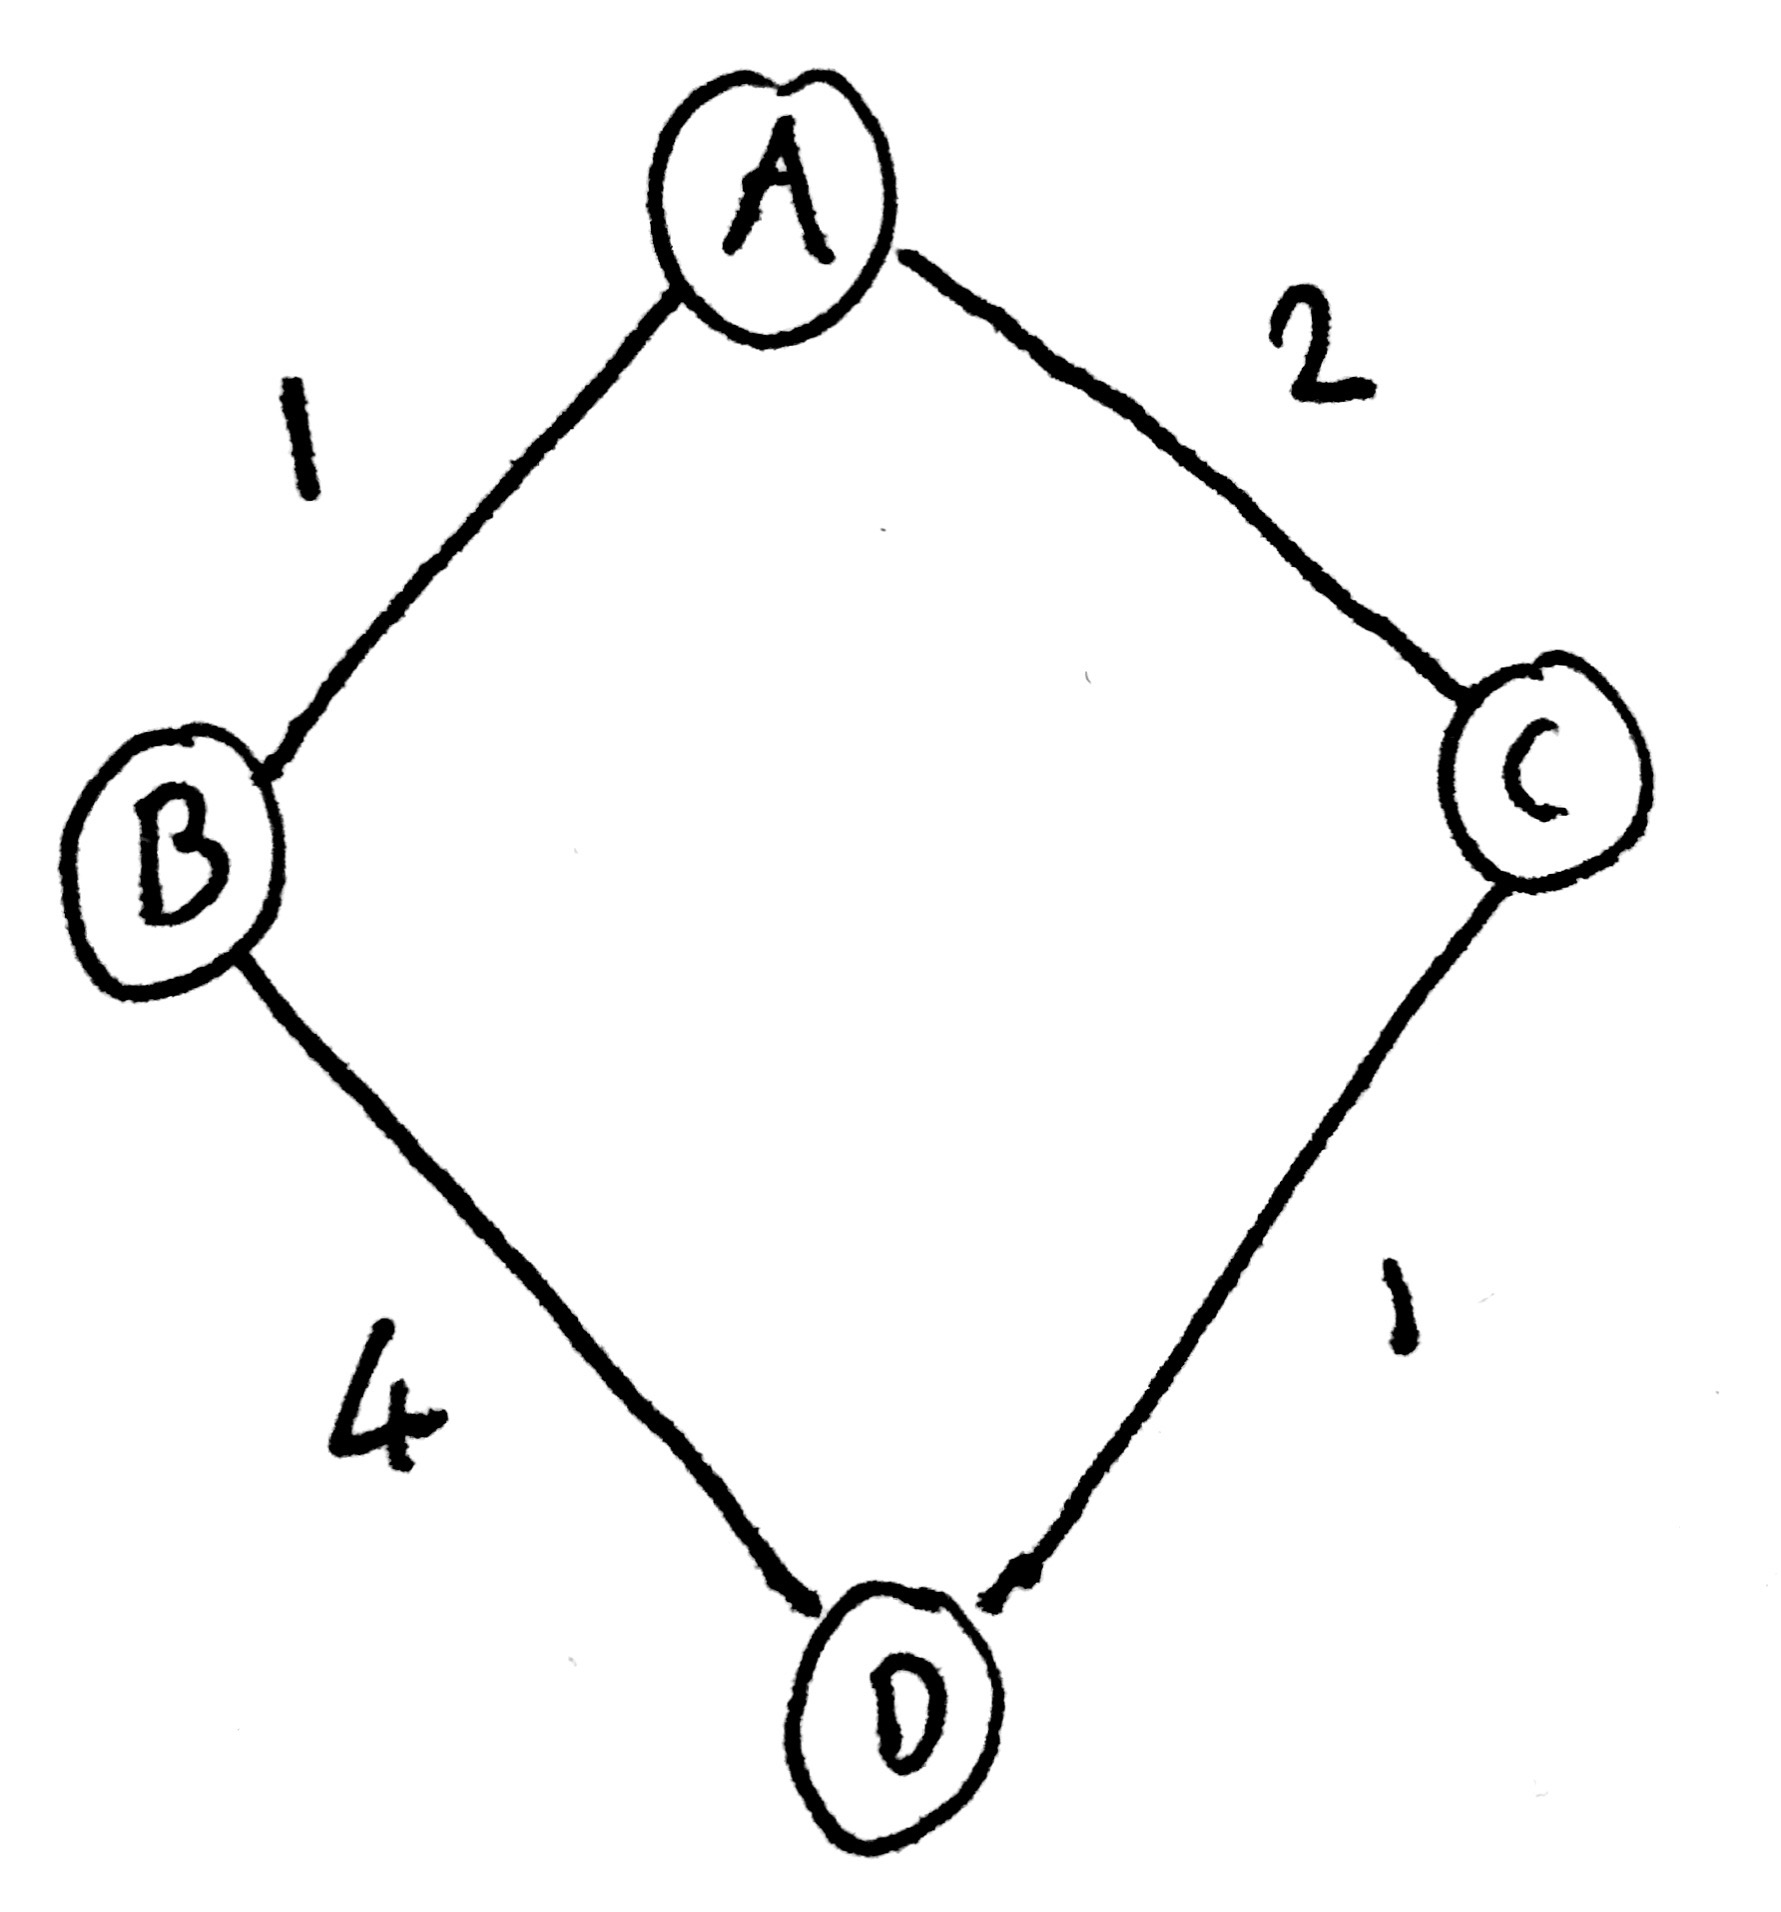
\includegraphics[width=0.6\textwidth]{1-tree}
        \end{center}

        In this example, if searching for an optimal path from $A$ to $D$, $B$
        will be expanded. If a goal test is performed on its descendants then
        the algorithm will terminate since $D$ is a descendant despite the fact
        that this is not the optimal path.

        \emph{Not sure about other reason}
      \end{solution}

    \question The $f$-cost is defined in the usual way as:
      \begin{center}
        $f(n) = p(n) + h(n)$
      \end{center}

      where $n$ is any node, $p$ denotes path cost and $h$ denotes the
      heuristic. An admissible heuristic is one for which, for any $n$

      \begin{center}
        $h(n) \leq$ actual distance from $n$ to the goal
      \end{center}

      and a heuristic is monotonic if for consecutive nodes $n$ and $n'$ it is
      always the case that

      \begin{center}
        $f(n') \geq f(n)$.
      \end{center}

      \begin{parts}
        \part Prove that $h$ is monotonic if and only if it obeys the triangle
          inequality, which states that for any consecutive nodes $n$ and $n'$

          \begin{center}
            $h(n) \leq c_{n \rightarrow n'} + h(n')$
          \end{center}

          \begin{solution}
            \begin{align*}
              f(n)  &= p(n) + h(n) \\
              f(n') &= p(n') + h(n') = p(n) + c_{n \rightarrow n'} + h(n')
            \end{align*}

            If the triangle inequality is satisfied we have:

            \begin{equation*}
              h(n) \leq c_{n \rightarrow n'} + h(n')
            \end{equation*}

            and thus we have:

            \begin{equation*}
              p(n) + h(n) \leq p(n) + c_{n \rightarrow n'} + h(n')
            \end{equation*}

            Therefore:

            \begin{equation*}
              f(n) \leq f(n')
            \end{equation*}

            The reverse implication is similar, starting with $f(n) \leq f(n')$,
            expand out and cancel the $p(n)$ to be left with the triangle
            inequality.
          \end{solution}

        \part Prove that if a heuristic is monotonic then it is also admissible.

          \begin{solution}
            There are two cases, either the goal is reachable or it isn't.

            \begin{description}
              \item[Case where goal is unreachable] In this case the actual
                distance is infinite and thus anything is admissible since it
                is not possible to overestimate the distance.

              \item[Case where goal is reachable] If the heuristic is monotonic
                then we have:

                \begin{equation*}
                  f(n) \leq f(n')
                \end{equation*}

                Expanding this gives us

                \begin{align}
                  p(n) + h(n) &\leq p(n') + h(n') \\
                  p(n) + h(n) &\leq p(n) + c_{n \rightarrow n'} + h(n') \\
                  h(n) &\leq c_{n \rightarrow n'} + h(n') \label{eq:1}
                \end{align}

                Since $h(n_{goal})$ is defined to be zero, for the node
                preceding the goal in the path we have:

                \begin{equation}
                  h(n) \leq c_{n \rightarrow n_{goal}} \label{eq:2}
                \end{equation}

                Using \eqref{eq:2} as the base case and performing induction
                using \eqref{eq:1}, it can be seen that \eqref{eq:2} holds for
                any node $n$. This inequality is the requirement for
                admissibility.

            \end{description}
          \end{solution}

        \part Is the converse true? (That is, are all admissible heuristics also
          monotonic?) Either prove that this is the case or provide a
          counterexample.

          \begin{solution}
            The converse is not true, a counterexample is a tree with 3 nodes,
            $X$, $Y$ and $Z$. The path costs are $C_{X \rightarrow Y} = 1$ and
            $C_{Y \rightarrow Z} = 2$. Let $h(X) = 3$ and $h(Y) = 1$.

            The heuristic is admissible since it never overestimates the
            distance, however it is not monotonic as $f(X) = 3$ and $f(Y)=2$,
            and thus $f(n) \leq f(n')$ does not hold.
          \end{solution}

      \end{parts}

    \question In RBFS we are replacing $f$ values every time we backtrack to
      explore the current best alternative. This seems to imply a need to
      remember the new $f$ values for all the nodes in the path we're
      discarding, and this in turn suggests a potentially exponential memory
      requirement. Why is this not the case?

      \begin{solution}
        \emph{Not sure}
      \end{solution}

    \section*{Games}

    \SetQuestionNumber{1}
    \question Consider the following game tree:
      \begin{center}
        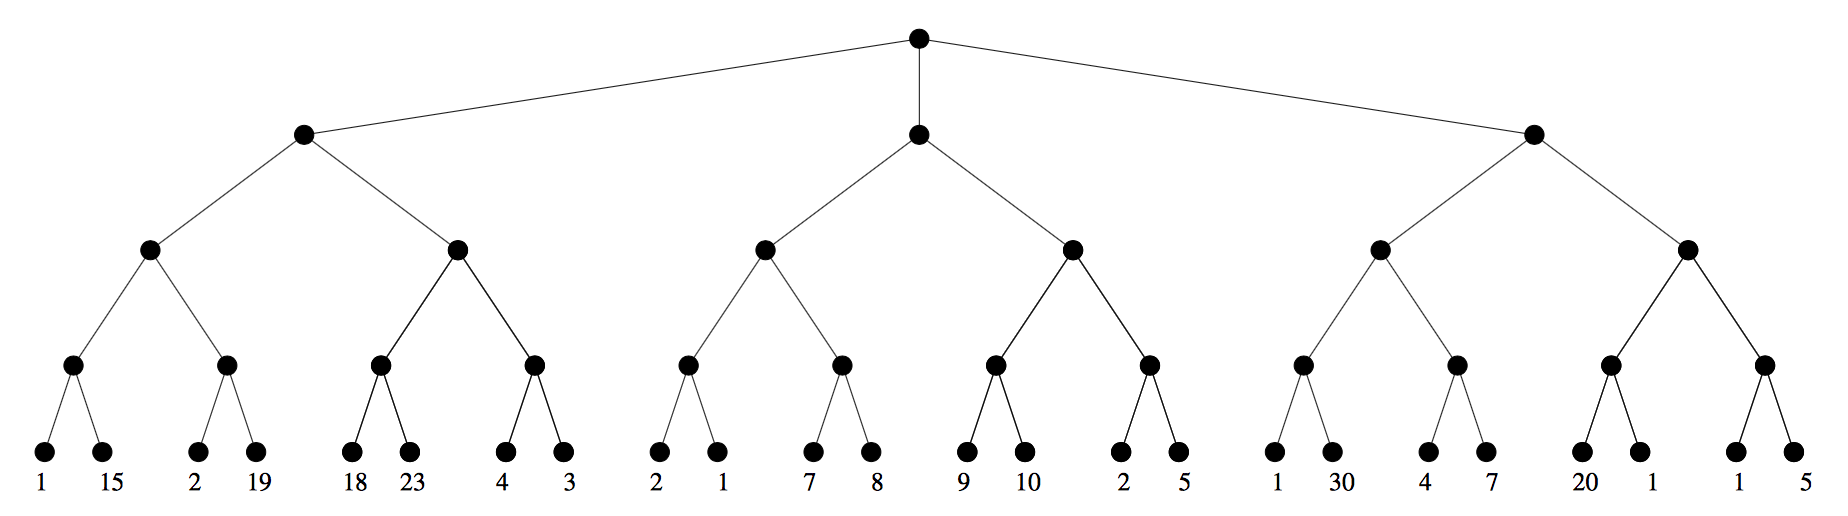
\includegraphics[width=0.9\textwidth]{1-graph}
      \end{center}

      Large outcomes are beneficial for Max. How is this tree pruned by $\alpha
      - \beta$ minimax if Max moves first? (That is, Max is the root.) How is it
      pruned if Min is the root, and therefore moves first?

      \begin{solution}
        I'm labelling sub trees using $M$, $L$ and $R$ to indicate middle, left
        and right respectively.

        The pruned subtrees are:

        \begin{itemize}
          \item $LR$
          \item $CLL$
          \item $CR$
          \item $RLL$
          \item $RLR$
          \item $R$
        \end{itemize}
      \end{solution}

    \question Implement the $\alpha - \beta$ pruning algorithm and use it to
      verify your answer to the previous problem.

    \question Is the minimax approach to playing games optimal against an
      imperfect opponent? Either prove this is the case or give a
      counterexample.

      \begin{solution}
        No it isn't, assume that the opponent always chooses the opposite of
        what it should. The following tree would result in a non-optimal result.

        \begin{code}{{}}

             / \
            /   \
           /\  / \
          1 10 2  3
        \end{code}
      \end{solution}

  \end{questions}
\end{document}
